\chapter{Optimization Algorithms}

\section{Reviewing}
\begin{itemize}
\item
In order to reach $\sqrt{\epsilon}$-FOSP such that $\|\nabla f(\theta^r)\|^2\le\epsilon$, 
the $\mathcal{O}(1/\epsilon)$ iterations are needed.
\item
Observe that each update of gradient descent is equivalent to minimizing a taylor-expansion-based quadratic upper bound on the objective function:
\[
x^{k+1}=x^k-t_k\nabla f(x^k)=\arg\min_{x\in\mathcal{X}}\frac{1}{2t_k}\|x-x^k\|^2+\nabla\trans f(x^k)(x-x^k).
\]
Therefore, gradient descent is one special case of successive convex approximation~(SCA) technique.
See the survey paper \citep{Razaviyayn2014SuccessiveCA} on the SCA technique for detail.
\end{itemize}


\section{Variants of Gradient Descent~(GD) Method}
\subsection{Scaled GD}
Consider the minimization problem
\[
\min_{\theta}F(\theta).
\]
The intuition of the scaled GD is to left-multiply the gradient $\nabla F(\theta_t)$ with a positive definite matrix to avoid osillation:
\[
\begin{array}{ll}
\theta_{t+1} = \theta_t - \alpha_tD_t\nabla F(\theta_t),
&
D_t\succ0.
\end{array}
\]

\begin{example}
Consider the linear regression problem
\begin{equation}\label{Eq:9:1}
\min_{\theta}~\frac{1}{2}\|A\theta - b\|^2,
\end{equation}
with 
\begin{align*}
A&=\begin{pmatrix}
a_1&\cdots&a_d
\end{pmatrix},\\
\theta &= (\theta_i)_{i=1}^d.
\end{align*}
In practice, the size for the feature $a_1$ can be very differnt from that of $a_2$.
In order to resolve this issue, the data transformation technique is applied, i.e., 
introduce a new variable
\[
w \triangleq S\theta,\qquad\text{where }S=\diag(s_1,\dots,s_d).
\]
It suffices to solve the new problem where the data matrix $AS^{-1}$ is well-conditioned:
\begin{equation}\label{Eq:9:2}
\min_{w}\|A S^{-1}W - b\|^2
\end{equation}
\begin{itemize}
\item
The GD method for solving (\ref{Eq:9:1}) is given by
\[
\theta_{t+1} = \theta_t - \gamma A\trans (A\theta_t -b)
\]
\item
The GD method for solving the transformed problem (\ref{Eq:9:2}) is given by
\[
w_{t+1}  =w_t - \gamma S^{-1}A\trans(AS^{-1}w_t - b)
\]
Left-multiplying $S^{-1}$ for this iteration gives
\[
\theta_{t+1} = \theta_t - \gamma S^{-2}A\trans (A\theta_t - b)
\]
\end{itemize}
Therefore, solving the transformed problem (\ref{Eq:9:2}) is equivalent to the scaled GD method by setting $D\equiv S^{-2}$.
\end{example}

\begin{example}[Newton's Method]
Newton's method is a special case of scaled GD by setting $D_t\equiv (\nabla^2 F(\theta_t))^{-1}$:
\[
\theta_{t+1} = \theta_t - \alpha_t(\nabla^2 F(\theta_t))^{-1}\nabla F(\theta_t)
\]
Newton's method performs good in linear regression problem. If we choose $\alpha_t=1$, then Newton's method gives the optimal solution in one iteration:
\begin{align*}
\theta_{t+1} &= \theta_t - \alpha_t(\nabla^2 F(\theta_t))^{-1}\nabla F(\theta_t)\\
&=\theta_t - (A\trans A)^{-1}\cdot[A\trans(A\theta - b)]\\
&=(A\trans A)^{-1}A\trans b.
\end{align*}
\end{example}

\begin{example}[Gauss-Newton Method]
Consider the non-linear regression problem
\[
\min_{\theta}~F(\theta)\triangleq \frac{1}{2}\sum_{i=1}^n[f_i(\theta)]^2
\]
The gradient and Hessian are computed as follows:
\begin{align*}
\nabla F(\theta) &= \sum_{i=1}^nf_i(\theta)\nabla_{\theta}f_i(\theta)\\
\nabla^2F(\theta)&=\sum_{i=1}^n\nabla_{\theta}f_i(\theta)\nabla\trans_{\theta}f_i(\theta)
+\underbrace{\sum_{i=1}^nf_i(\theta)\nabla^2f_i(\theta)}_{S(\theta)}
\end{align*}
The Gauss-Newton method sets 
\[
D_t\equiv\left(\sum_{i=1}^n\nabla_{\theta}f_i(\theta)\nabla\trans_{\theta}f_i(\theta)\right)^{-1},
\]
 which is an approximation of the inverse of the Hessian matrix.
 There are two advantages:
\begin{enumerate}
\item
It reduces the Hessian computation time into gradient computation time.
\item
The $D_t$ is positive definite, which avoids the numerical instability of Newton's method.
Actually, in the paper \citep{Zhang2000}, Prof. Yin Zhang compares the difference between these two methods. He found that the Gauss-Newton method possesses a desirable behavior of only seeking global (or good local) minima, while the Newton method is blindly attracted to all kinds of FOSPs. 


\end{enumerate}

\end{example}


\begin{remark}
There are generally two choices of step size for GD and variants of GD method:
\begin{itemize}
\item
Constant step size: $\alpha_t \in(0,1/L)$;
\item
Diminishing stepsize: $\alpha_t\to0$ but satisfies the infinite travel condition
\[
\sum_{t=1}^\infty\alpha_t=\infty.
\]
\end{itemize}
For constrained minimization problem, the projected gradient descent method is applied.
\end{remark}

\subsection{Stochastic Gradient Descent~(SGD)}
Consider minimizing an objective with the finite-sum form:
\[
F(\theta) = \frac{1}{N}\sum_{i=1}^N\ell(f_{\theta}(x_i),y_i) \triangleq \frac{1}{N}\sum_{i=1}^NF_i(\theta)
\]
The SGD iteration is given by 
\[
\theta_{t+1} = \theta_t -\alpha_t\nabla F_{j[t]}(\theta_t),
\]
where $j[t]$ is the sample randomly picked from $\{1,\dots,N\}$ at the $t$-th iteration.
\begin{remark}
\begin{enumerate}
\item
The SGD works under the following assumptions:
\begin{itemize}
\item
Each component function $F_i$ is Lipschitz continuous, i.e., $\|\nabla F_i(\theta) - \nabla F_i(\xi)\|\le L\cdot\|\theta - \xi\|$;
\item
The variance for estimation of gradient is uniformly bounded:
\[
\mathbb{E}\bigg[\|\nabla F_{j[t]}(x) - \nabla f(x)\|^2\bigg]\le\sigma^2
\]
\end{itemize}
\item
Stochastic gradient method is not a descent method, though it is frequently referred to as stochastic gradient descent in the literature.
\item
We will show that $\alpha_t$ has to be a dimishing step-size.
\item
If $j[t]$ are selected like the form $\{1,\dots,N,1\dots,N,\dots\}$, then it reduces to the incremental gradient algorithm.
\item
People prefer to use SGD in machine learning field instead of GD. 
The disadvantage for SGD is that it needs $\mathcal{O}(1/\epsilon^2)$ iterations to get $\sqrt{\epsilon}$-FOSP, while GD needs only $\mathcal{O}(1/\epsilon)$ iterations.
However, the complexity of the number of gradient calls in each inner iteration is different. 
The computation of the gradient of component functions per iteration for SGD is $\mathcal{O}(1)$, but GD requires $\mathcal{O}(N)$ calls. 
Due to this fact, SGD is faster than GD in practice.
\begin{center}
\begin{table}[H]
\centering
\begin{tabular}{|c|c|c|}
\hline
 				   & $\#$ gradient calls per iteration & $\#$ iterations   \\
 				   \hline
 GD   & $n$   &     $\bm {\epsilon^{-1}}$  \\
 \hline
 SGD   & $\bm 1$   &    $\epsilon^{-2}$  \\
  \hline
\end{tabular}
\caption{Comparison of SGD and GD
}
\end{table}
\end{center}

\end{enumerate}
\end{remark}
\begin{theorem}
Suppose that the objective function satisfies the assumptions mentioned before, and the SGD is applied in each iteration:
\[
\theta_{t+1} = \theta_t-\alpha_tg_t,\qquad
\text{where }g_t:=\nabla F_{j[t]}(\theta_t).
\]
Define $T^*:=\min\{i: \|\nabla F(\theta_i)\|^2\le\epsilon\}$, then $T^*=\mathcal{O}(1/\epsilon^2)$. 
\end{theorem}

\begin{proof}
\begin{enumerate}
\item
Step 1: SGD always makes significant progess in each iteration.
\begin{align*}
F(\theta_{t+1})&\le F(\theta_t)+\inp{\nabla F(\theta_t)}{\theta_{t+1} - \theta_t} + \frac{L}{2}\|\theta_{t+1} - \theta_t\|^2\\
&=F(\theta_t)-\alpha_t\inp{\nabla F(\theta_t)}{g_t}+\frac{L\alpha_t^2}{2}\|g_t\|^2
\end{align*}
Then taking conditional expectation both sides given $\theta_t$ leads to
\begin{equation}\label{Eq:9:3}
\begin{aligned}
\mathbb{E}[F(\theta_{t+1})\mid \theta_t]&\le F(\theta_t)-\alpha_t\inp{\nabla F(\theta_t)}{\mathbb{E}[g_t\mid\theta_t]}+\frac{L\alpha_t^2}{2}\mathbb{E}[\|g_t\|^2\mid\theta_t]\\
&=F(\theta_t)-\alpha_t\|\nabla F(\theta_t)\|^2+\frac{L\alpha_t^2}{2}\mathbb{E}[\|g_t\|^2\mid\theta_t]
\end{aligned}
\end{equation}
Furthermore, by the equality $\|a\|^2\le 2\|a-b\|^2+2\|b\|^2$,
\begin{align*}
\mathbb{E}[\|g_t\|^2\mid\theta_t]&\le 2\mathbb{E}[\|g_t-\nabla F(\theta_t)\|^2\mid\theta_t]+2\|\nabla F(\theta_t)\|^2\\&
=2\sigma^2+2\|\nabla F(\theta_t)\|^2
\end{align*}
Substituting this identity into the RHS of (\ref{Eq:9:3}) gives
\begin{align*}
\mathbb{E}[F(\theta_{t+1})\mid \theta_t]&\le 
F(\theta_t)+\left(-\alpha_t+L\alpha_t^2\right)\|\nabla F(\theta_t)\|^2+L\alpha_t^2\sigma^2\\
&\le F(\theta_t)-\frac{\alpha_t}{2}\|\nabla F(\theta_t)\|^2+L\alpha_t^2\sigma^2
\end{align*}
where the last inequality is by choosing sufficiently small $\alpha_t$.
Therefore, the expected decrease in each iteration is bounded by the gradient term plus some variance:
\[
\mathbb{E}[F(\theta_{t+1})]-\mathbb{E}[F(\theta_{t})]\le -\frac{\alpha_t}{2}\|\nabla F(\theta_t)\|^2+L\alpha_t^2\sigma^2
\]
\item
Step 2: 
Considering the best performance in the first $T^*$ iteration.

Suppose that the step size $\alpha_t\equiv\alpha$ for all $t$. Then summing over the inequality above for $t=1,\dots,T^*$ gives
\begin{align*}
\frac{1}{T^*}\sum_{t=0}^{T^*}\mathbb{E}[\|\nabla F(\theta_t)\|^2]&\le \frac{2\mathbb{E}[F(\theta_0) - F(\theta_{T^*+1})]}{\alpha T^*}+2L\alpha\sigma^2\\
&\le \frac{2[F(\theta_0) - F(\theta_{\infty})]}{\alpha T^*}+2L\sigma^2\alpha 
\end{align*}
%Moreover, since $T^*$ is the first iteration where the iterate reaches the $\sqrt{\epsilon}$-suboptimality point,
%\begin{align*}
%\epsilon\frac{\alpha}{2}&\le \frac{1}{T^*}\sum_{t=0}^{T^*}\frac{\alpha}{2}\mathbb{E}[\|\nabla F(\theta_t)\|^2]\le [F(\theta_0) - F(\theta_{\infty})]+L\alpha^2\sigma^2T^*
%\end{align*}
Choosing $\alpha=1/\sqrt{T}$ gives
\[
\frac{1}{T^*}\sum_{t=0}^{T^*}\mathbb{E}[\|\nabla F(\theta_t)\|^2]
\le \frac{2[F(\theta_0) - F(\theta_{\infty})]+2L\sigma^2}{\sqrt{T^*}}
\]
Moreover, since $T^*$ is the first iteration where the iterate reaches the $\epsilon$-suboptimality point,
\[
\epsilon\le \frac{1}{T^*}\sum_{t=0}^{T^*}\mathbb{E}[\|\nabla F(\theta_t)\|^2]\le \frac{2[F(\theta_0) - F(\theta_{\infty})]+2L\sigma^2}{\sqrt{T^*}}
\]
Or equivalently,
\[
T^*\le \frac{2[F(\theta_0) - F(\theta_{\infty})]+2L\sigma^2}{\epsilon^2}=\mathcal{O}(\epsilon^{-2}).
\]
\end{enumerate}
\end{proof}


\section{Momentum-based Method}
Now we introduce several famous momentum methods. 
\subsection{Heavy-Ball Method}
Each update of Heavy-Ball Method uses the information from the last and the last second iterate points:
\[
\left\{
\begin{aligned}
m_t &=\beta m _{t-1} + (1-\beta)\nabla F(\theta_t)\\
\theta_{t+1}&=\theta_t - \alpha_tm_t
\end{aligned}
\right.
\]
\begin{remark}
For convex objective function, the heavy-ball method can accelerate the convergence rate from $\mathcal{O}(1/\epsilon)$ iterations into $\mathcal{O}(1/\sqrt{\epsilon})$ iterations.
However, it is not clear how the heavy-ball method behaves in general non-convex problems.
\end{remark}
\subsection{Adaptive Gradient methods~(AdaGrad)~\citep{Duchi2001}}
The AdaGrad can be viewed as a scaled version of the SGD:
\[
\begin{array}{ll}
&\theta_{t+1} = \theta_t - \alpha_t(D^t)^{-1/2}g_t,\\
\text{where}&D^t = \frac{1}{t}\sum_{s=1}^tg_s\cdot g_s\trans
\end{array}
\]
The inituition is that the step size of SGD is hard to control. 
The AdaGrad resolves this issue by rescaling the step size of $i$-th coordinate
from $\alpha_t$ to $\frac{\alpha_t}{\sqrt{\frac{1}{t}\sum_{s=1}^tg_ig_j}}$
In practice, the inverse of $D^t$ is difficult to compute, and therefore we approximate its inverse by simply inversing the diagonal entries of $D^t$:
\[
\theta_{t+1} = \theta_t - \alpha_t \diag\left(
\frac{1}{t}\sum_{s=1}^tg_s\cdot g_s\trans
\right)^{-1/2}g_t
\]
Or equivalently, this iteration can be written as
\[
\left\{
\begin{aligned}
v_t &= \frac{1}{t}\sum_{s=0}^tg_s\circ g_s\\
\theta_{t+1} &=  \theta_t - \alpha_t (v^t)^{-1/2}\circ g_t
\end{aligned}
\right.
\]

\subsection{RMS-Prop~\citep{RMSProp}}
The RMSprop algorithm is a variant version of AdaGrad, by doing exponential decay of previous information $v_{t-1}$:
\[
\left\{
\begin{aligned}
v_t &=\beta v_{t-1} + (1-\beta)g_t\circ g_t\\
\theta_{t+1} &=  \theta_t - \alpha_t (v^t)^{-1/2}\circ g_t
\end{aligned}
\right.
\]
\begin{remark}
Unfortunately, there is no theory concerning how to choose $\beta$ optimally in literature.
\end{remark}

\subsection{Adam~\citep{kingma-adam}}
Finally, let's introduce the Adam algorithm, which not simply enjoys features from heavy-ball method such that the gradient estimate is momentum, but also borrows ideas from RMSprop such that the step size is adaptively chosen with exponential decay.
\[
\left\{
\begin{aligned}
m_t&=\beta_1 m_{t-1} + (1-\beta_1)g_t\\
v_t&=\beta_2v_{t-1} + (1-\beta_2)g_t\circ g_t\\
\theta_{t+1}&=\theta_t - \alpha_tv_t^{-1/2}\circ m_t
\end{aligned}
\right.
\]
\paragraph{Bibliography}
In 2018 ICLR, the paper \citep{2018on} gives a counter-example to show that Adam does not converge for convex problems.
Specifically, consider the problem
\[
\min_{\theta}F(\theta)=\sum_{j=1}^nF_j(\theta),
\]
with 
\[
F_j(\theta) = \left\{
\begin{aligned}
5.5\theta^2,&\quad j=1\\
-0.5\theta^2,&\quad j\ne1
\end{aligned}
\right.
\]
The special parameter of Adam $\beta_1=0,\beta_2=1$ gives the signSGD:
\[
\theta_{t+1} = \theta_t - \alpha_t \text{sign}(g_t)
\]
which is unlikely to converge.
Then they propose AMSGrad to correct this algorithm.
Later in 2019 ICLR, the paper \citep{chen2018on} shows that Adam-type algorithms do not converge for non-convex problems, and they propose the AdaFom to correct previous algorithms' behaviors.

\paragraph{Summary}
The Adam-Type Method can be expressed as follows:
\[
\left\{
\begin{aligned}
m_t &= \beta_{1,t} m_{t-1} + (1-\beta_{1,t})g_t\\
\hat{v}_t &= h_t(g_1,\dots,g_t)\\
\theta_{t+1} &= \theta_t - \alpha_tm_t/\sqrt{\hat{v}_t }
\end{aligned}
\right.
\]
Some popular variants of the Adam algorithm is shown in the Table below:
\begin{figure}[H]
\centering
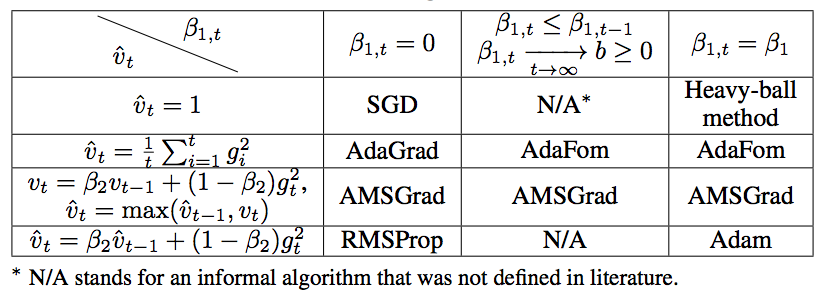
\includegraphics[width=\textwidth]{Nineth_lecture/p_6}
\caption{Variants of Adam algorithm}
\end{figure}




\section{Nonconvex nonconcave minimax optimization}
Consider the minimax problem
\[
\min_x\max_yf(x,y)
\]
If we can obtain $y^*=h(x)$, then it suffices to solve the minimization problem
\[
\min_xg(x)\triangleq f(x,h(x)).
\]
In practice, the function $g(x)$ is always defined implicitly.
This problem is the basis of generative adversarial networks and robust training.
The gradient descent ascent~(GDA) Algorithm is widely used in this problem, but this algorithm cannot even solve a linear problem
\[
\min_x\max_y x\trans Ay.
\]
\begin{remark}
\begin{enumerate}
\item
Now there are two state-of-the-art algorithms for solving the minimax problem. The first one is the optimistic GDA; and the second one is to applying BCD heuristic, i.e., approximately optimizing the inner problem in terms of $y$ for few iterations, and then perform gradient descent for the outer problem for one iteration.
The assumptions for the second algorithm is that the problem in terms of $y$ is concave, and the constraint set is bounded.
\item
It is even not clear what is the local optimality for the minimax problem in the general setting.
\item
The GDA is widely used, but its convergence properties remain to be understood.
\end{enumerate}
\end{remark}

